\clearpage
\section{Task Description}
\label{sec:appx_task_desc}
\benchname\xspace is constructed using a carefully designed taxonomy to evaluate four types of memory: temporal, spatial, object, and procedural. These memory types correspond to four task suites, \TSone, \TStwo, \TSthree, and \TSfour, respectively, each comprising four tasks.

Across all tasks, the environments use a fixed set of tabletop objects (see Fig.~\ref{fig:basic_objets}), grouped by their functional roles:

\begin{itemize}
    \item \textbf{Primitive Objects:}
    \begin{itemize}
        \item \textbf{Cubes} (green/blue/red) for basic pick-and-place manipulation.
        \item \textbf{Pegs} for insertion in the \textit{InsertPeg} task.
        \item \textbf{Hook stick} for pulling or repositioning objects in the \textit{MoveCube} task.
        \item \textbf{Routing stick} for navigating around obstacles in the \textit{RouteStick} task.
        \item \textbf{Highlighted areas}, implemented as white discs beneath objects, that provide temporary visual cues in the \textit{PickHighlight} task.
    \end{itemize}

    \item \textbf{Interactive Objects:}
    \begin{itemize}
        \item \textbf{Targets}, colored discs (purple/red/gray) that change color to indicate state transitions.
        \item \textbf{Buttons} for press-based interaction, typically serving as termination signals.
    \end{itemize}

    \item \textbf{Specialized Receptacles:}
    \begin{itemize}
        \item \textbf{Containers} that can be picked up to cover and hide cubes, testing spatial memory.
        \item \textbf{Aperture box} (box with a hole) for peg insertion tasks.
        \item \textbf{Opaque bin} with a black interior for the \textit{BinFill} task, preventing visual counting and enforcing object-permanence reasoning.
    \end{itemize}
\end{itemize}




Detailed descriptions of each task are provided below.

\begin{figure}
    \centering
    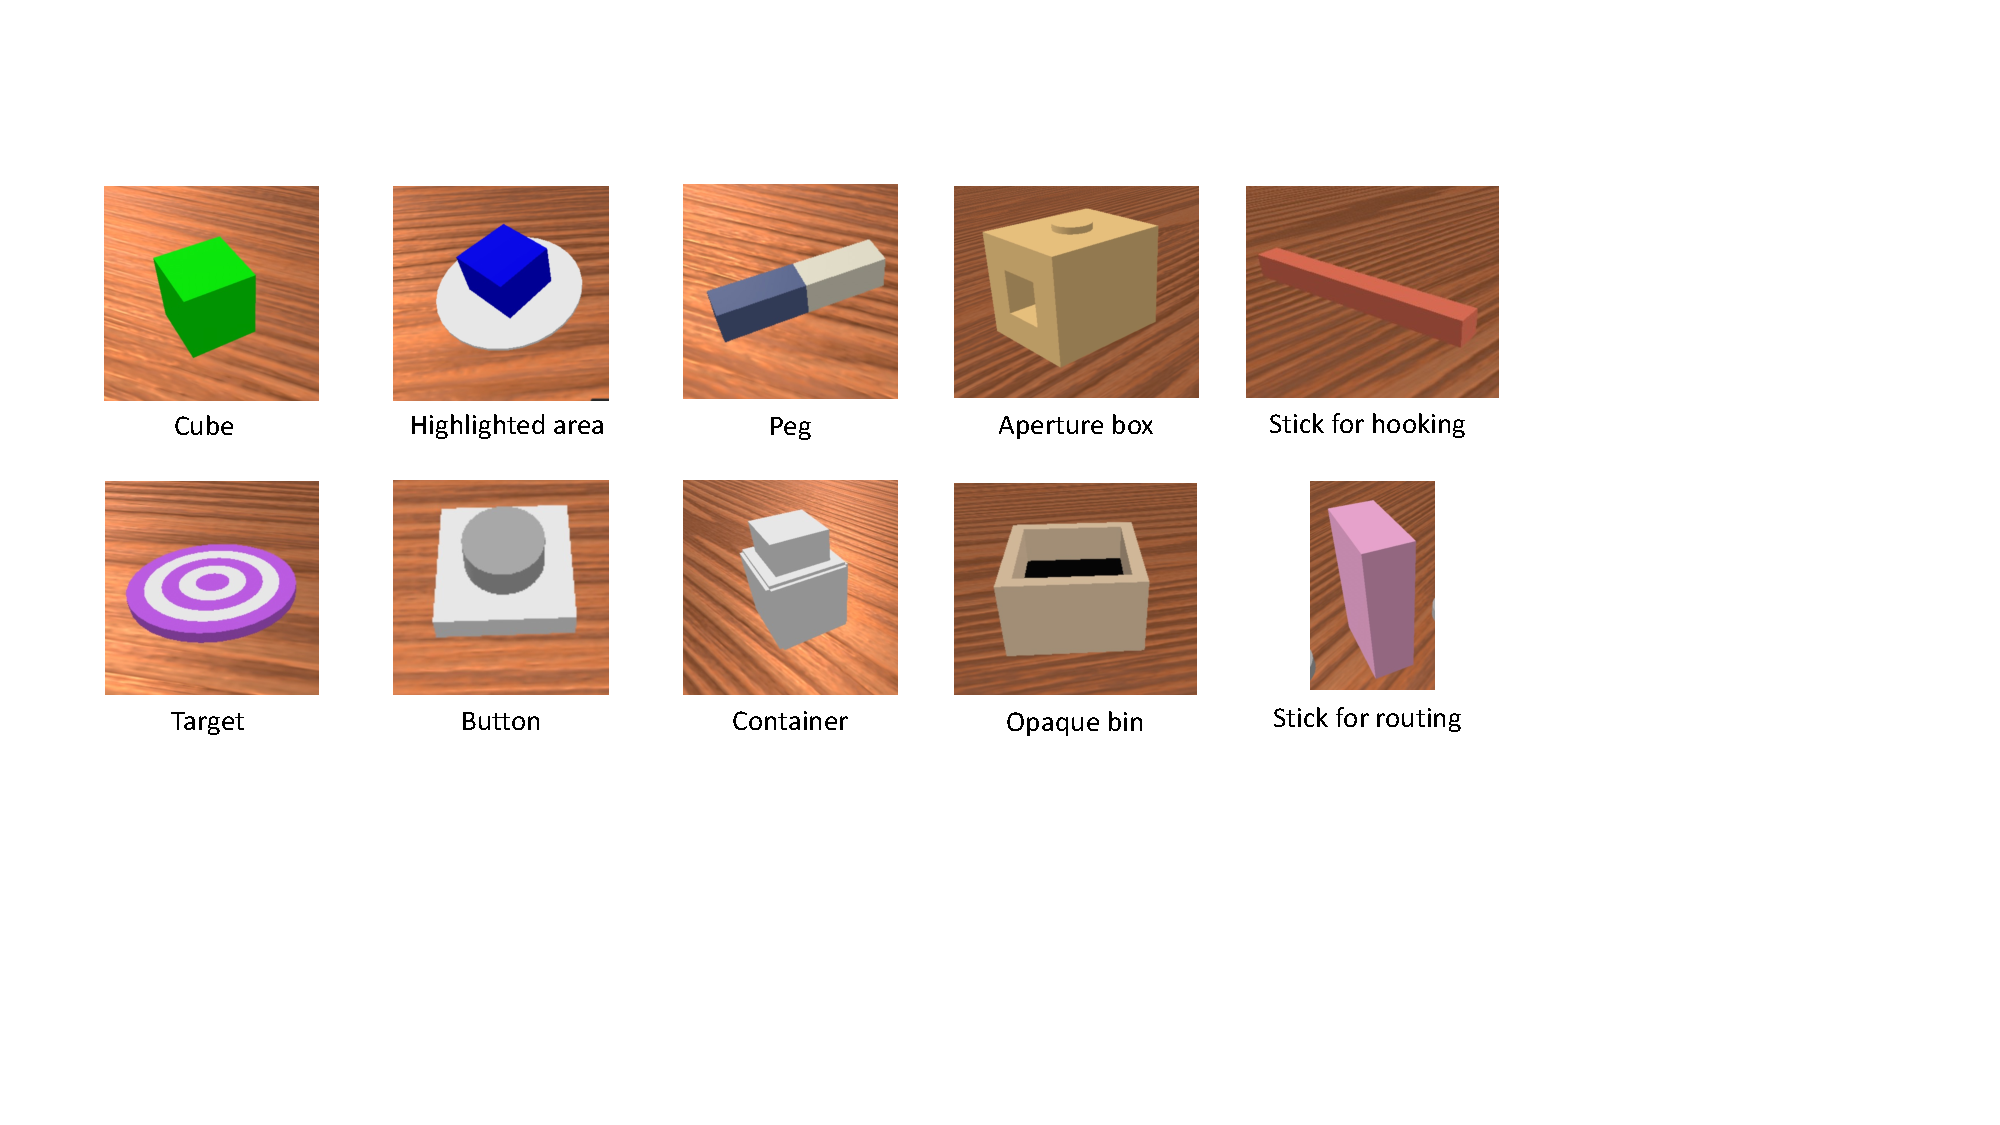
\includegraphics[width=0.9\linewidth]{images/basic_objects2.pdf}
    \caption{Overview of the main assets used in RoboMME.}
    \label{fig:basic_objets}
\end{figure}


\clearpage

\subsection{BinFill}
\label{sec:task_binfill}

\begin{wraptable}{r}{0.35\linewidth}
    \centering
    \caption{\textit{BinFill} Task Configuration.}
    \label{tab:binfill_difficulty_config}
    \renewcommand{\arraystretch}{1.2}
   {\resizebox{\linewidth}{!}{
    \begin{tabular}{l c c c}
        \toprule
        \textbf{Difficulty} & \textbf{\#Colors} & \textbf{\#Total Cubes} & \textbf{\#Goal Cubes} \\
        \midrule
        Easy   & 1 & 4--6  & 1 \\
        Medium & 2 & 8--10 & 1--2 \\
        Hard   & 3 & 10--12 & 2--3 \\
        \bottomrule
    \end{tabular}}}
\end{wraptable}


The \textit{BinFill} task, illustrated in Fig.~\ref{fig:binfill}, evaluates sequential decision-making and temporal memory. The robot must place a specified number of colored cubes into a bin and then press a button to terminate the episode. Success requires accurate counting and timely termination. Task configurations are summarized in Table~\ref{tab:binfill_difficulty_config}.

\begin{figure}
    \centering
    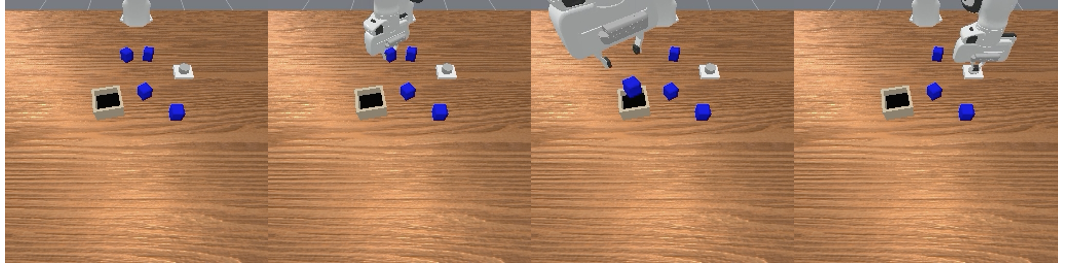
\includegraphics[width=0.9\linewidth]{images/tasks/binfill.png}
    \caption{\textbf{BinFill Task Example.} In this instance, the goal is to place one blue cube into the bin and then press the button to stop.}
    \label{fig:binfill}
\end{figure}


\paragraph{Language Goals}
We define three types of language instructions with increasing compositional complexity:
\begin{enumerate}[itemsep=1pt, topsep=0pt, leftmargin=*]
    \item Place \textbf{one} cube of a specified color.  
    \textit{e.g., ``put one blue cube into the bin and press the button to stop''}.
    
    \item Place cubes of \textbf{two} specified colors.
    \textit{e.g., ``put one blue cube and two green cubes into the bin and press the button to stop''}.
    
    \item Place cubes of \textbf{three} specified colors.
    \textit{e.g., ``put one blue cube, one green cube and two red cubes into the bin and press the button to stop''}.
\end{enumerate}

\paragraph{Task Characteristics}
To introduce dynamic and history-dependent behavior, we consider two settings randomly selected at environment initialization:
\begin{enumerate}[itemsep=1pt, topsep=0pt, leftmargin=*]
    \item \textbf{Static:} all cubes are present at the beginning of the episode.
    \item \textbf{Streaming:} cubes appear incrementally over time in a random order.
\end{enumerate}

\paragraph{Success Criteria}
\begin{itemize}[itemsep=1pt, topsep=0pt, leftmargin=*]
    \item \textbf{Correct completion:} the button is pressed only after the exact required number of cubes for each specfied color has been placed in the bin.
    \item \textbf{Failure:} placing fewer or more cubes than required for any color at evaluation time.
    \item \textbf{Immediate failure:} exceeding the required count for any color will terminate the episode early.
\end{itemize}



\clearpage


\subsection{PickXtimes}
\label{sec:task_pickxtimes}


\begin{wraptable}{r}{0.35\linewidth}
    \centering
    \centering
    \caption{\textit{PickXtimes} Task Configuration.}
    \label{tab:pickxtimes_difficulty_config}
    \renewcommand{\arraystretch}{1.2}
  {{\resizebox{\linewidth}{!}{
    \begin{tabular}{l c c}
        \toprule
        \textbf{Difficulty} & \textbf{\#Total Cubes} & \textbf{\#Repetitions} \\
        \midrule
        Easy   & 1 & 1--3 \\
        Medium & 3 (2 distractors) & 1--3 \\
        Hard   & 3 (2 distractors) & 4--5 \\
        \bottomrule
    \end{tabular}}}}
\end{wraptable}

The \textit{PickXTimes} task, illustrated in Fig.~\ref{fig:pickxtimes}, evaluates the robot’s ability to perform iterative pick-and-place actions with temporal memory. The robot repeatedly picks up a cube of a specified color, places it on a target, and completes an exact number of cycles before pressing a button to terminate the task.
% Successful completion requires long-horizon consistency and the ability to internally track progress against a language-specified count. 
Task configurations are summarized in Table~\ref{tab:pickxtimes_difficulty_config}.

\begin{figure}
    \centering
    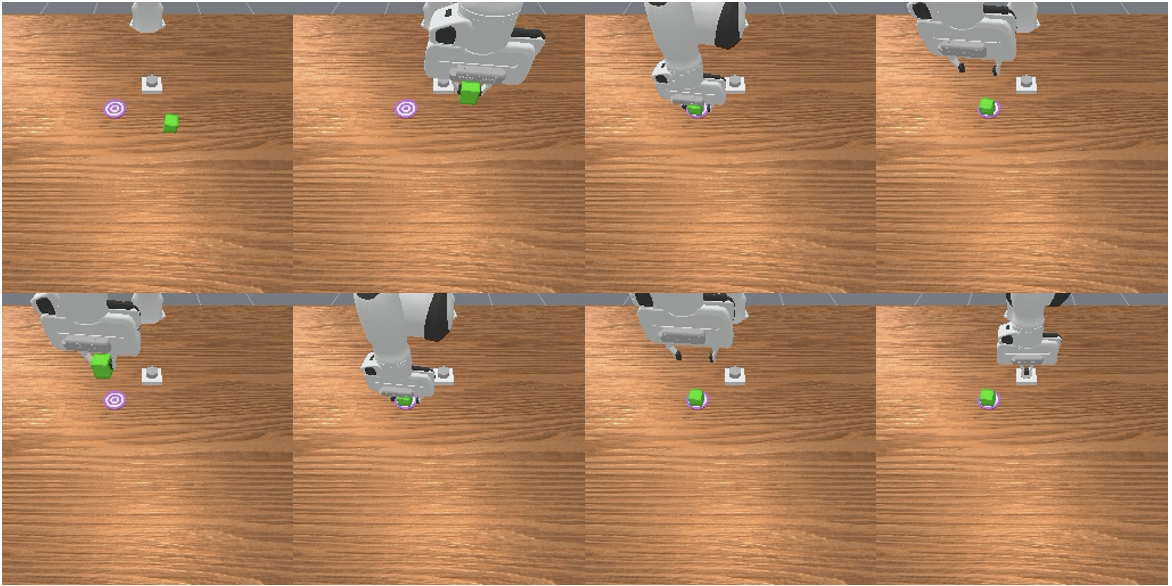
\includegraphics[width=0.8\linewidth]{images/tasks/pickxtimes.png}
    \caption{\textbf{PickXtimes Task Example.} In this instance, the goal is to pick up the green cube and place it on the target twice, then press the button to stop.}
    \label{fig:pickxtimes}
\end{figure}



\paragraph{Language Goals}
We define two types of language instructions:
\begin{enumerate}[itemsep=1pt, topsep=0pt, leftmargin=*]
    \item Pick and place for \textbf{one} time. 
    \textit{e.g., ``pick up the blue cube and place it on the target, then press the button to stop''}.
    
    \item Pick and place for \textbf{multiple} times.
    \textit{e.g., ``pick up the blue cube and place it on the target, repeating this pick-and-place action three times, then press the button to stop''}.

\end{enumerate}


\paragraph{Successful Pick-and-Place} A pick-and-place is considered successful when the robot lifts the cube above a predefined height threshold while maintaining a valid grasp, and then lowers it onto the target surface below a specified placement height.



\paragraph{Success Criteria}
\begin{itemize}[itemsep=1pt, topsep=0pt, leftmargin=*]
    \item \textbf{Correct completion:} the robot completes exactly the specified number of pick-and-place repetitions and then presses the button to terminate the episode.
    \item \textbf{Immediate failure:} The episode terminates early if:
        \begin{enumerate}[itemsep=1pt, topsep=0pt, leftmargin=*]
            \item The robot picks up a wrong cube.
            \item The button is pressed before all required repetitions are completed.
            \item The robot performs more pick-and-place repetitions than specified.
        \end{enumerate}
\end{itemize}

\clearpage



\subsection{SwingXtimes}
\label{sec:task_swingxtimes}

\begin{wraptable}{r}{0.35\linewidth}
    \centering
    \caption{\textit{SwingXtimes} Task Configuration.}
    \label{tab:swingxtimes_difficulty_config}
    \renewcommand{\arraystretch}{1.2}
 {   {\resizebox{\linewidth}{!}{
    \begin{tabular}{l c c}
        \toprule
        \textbf{Difficulty} & \textbf{\#Total Cubes} & \textbf{\#Repetitions} \\
        \midrule
        Easy   & 1 & 1--3 \\
        Medium & 3 (2 distractors) & 1--2 \\
        Hard   & 3  (2 distractors) & 3 \\
        \bottomrule
    \end{tabular}}}}
\end{wraptable}

The \textit{SwingXtimes} task is  illustrated in Fig.~\ref{fig:swingxtimes}. The robot must pick up a specified colored cube, transport it back and forth between two distinct targets (right-side and left-side) for a specified number of repetitions, and then press a button to stop. 
% Successful completion requires maintaining trajectory precision over extended manipulation sequences without accumulating errors. 
% Task configurations are given in Table~\ref{tab:swingxtimes_difficulty_config}.

\begin{figure}
    \centering
    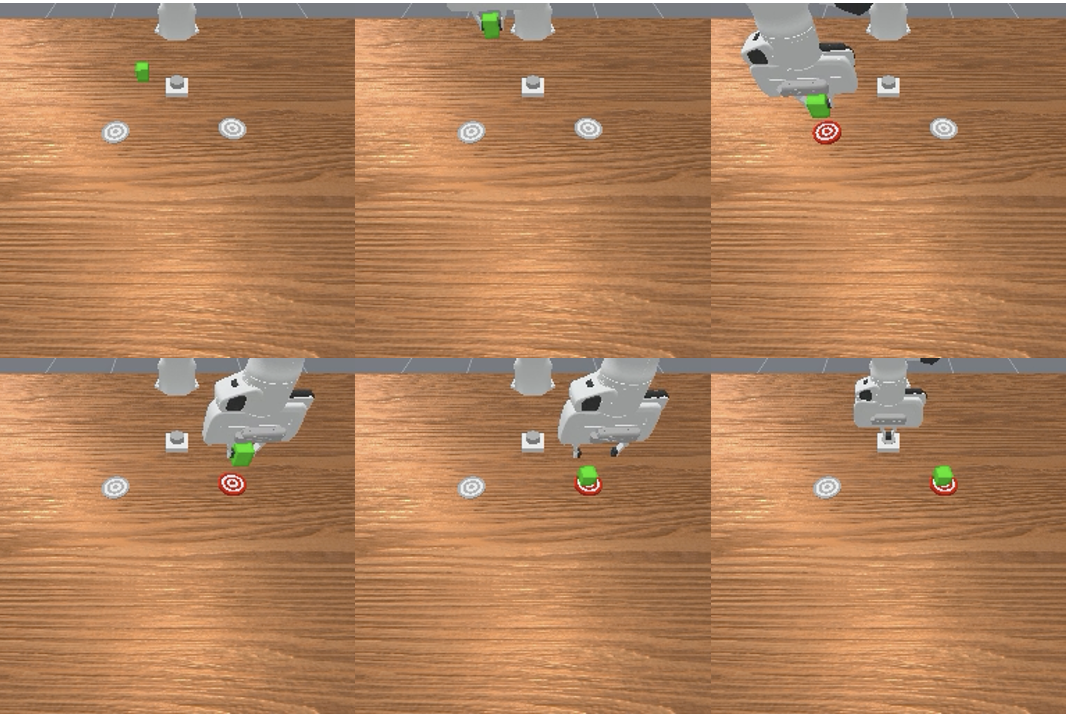
\includegraphics[width=0.6\linewidth]{images/tasks/swingxtimes.png}
    \caption{\textbf{SwingXtimes Task Example.} In this instance, the goal is pick up the green cube, first move it to the right-side target, then put down the cube on the left-side target (i.e., swing between targets one time), finally press the button to stop. Spatial directions (e.g., left/right) follow the robot base coordinate frame rather than the front camera frame.}
    \label{fig:swingxtimes}
\end{figure}



\paragraph{Language Goals}
We define two types of language instructions with increasing compositional complexity:
\begin{enumerate}[itemsep=1pt, topsep=0pt, leftmargin=*]
    \item Perform \textbf{one} swing cycle.
    \textit{e.g., ``Pick up the green cube, move it to the right-side target and then put down the cube on the left-side target and press the button to stop''}.

    \item Perform \textbf{multiple} swing cycles.
    \textit{e.g., ``Pick up the green cube, move it to the right-side target and then to the left-side target, repeating this right-to-left swing motion three times, then put down the cube and press the button to stop.''}.
\end{enumerate}

\paragraph{Successful Reach} A reach is successful when the cube is held nearly upright and positioned within a small tolerance of the target center in both vertical alignment and horizontal offset. Upon success, the target changes from gray to red, indicating that the gripper has reached it.


\paragraph{Success Criteria}
\begin{itemize}[itemsep=1pt, topsep=0pt, leftmargin=*]
    \item \textbf{Correct completion:} The button is pressed only after the robot completes the exact required number of swing motions between the two targets and places the cube on the table.
        
    \item \textbf{Immediate failure:} The episode terminates early if:
    \begin{enumerate}[itemsep=1pt, topsep=0pt, leftmargin=*]
        \item The robot picks up the wrong cube.
        \item The button is pressed before all repetitions are completed.
        \item The robot reaches either target more than the specified number of times (excessive swings).
    \end{enumerate}
\end{itemize}
\clearpage



\subsection{StopCube}
\label{sec:task_stopcube}


\begin{wraptable}{r}{0.35\linewidth}
    \centering
    \caption{\textit{StopCube} Task Configuration.}
    \label{tab:stopcube_difficulty_config}
    \renewcommand{\arraystretch}{1.2}
   {\resizebox{\linewidth}{!}{
    \begin{tabular}{l c c}
        \toprule
        \textbf{Difficulty} & \textbf{\#Passes} & \textbf{Move Speed} \\
        \midrule
        Easy   & 2--3 & slow/medium/fast \\
        Medium & 3--4 & slow/medium/fast \\
        Hard   & 4--5 & slow/medium/fast \\
        \bottomrule
    \end{tabular}}}
\end{wraptable}


The \textit{StopCube} task, illustrated in Fig.~\ref{fig:stopcube}, challenges the robot’s temporal memory in a dynamic environment. The robot must monitor a cube that continuously oscillates across a target following a predefined line and press a button to stop \textit{exactly} when the cube reaches the target at a specified ordinal occurrence (e.g., the third visit). Successful completion requires combining continuous visual tracking with discrete event counting to identify the correct occurrence and execute the stopping action with high temporal precision.
Detailed Task Configurations are summarized in Table.~\ref{tab:stopcube_difficulty_config}.

\begin{figure}
    \centering
    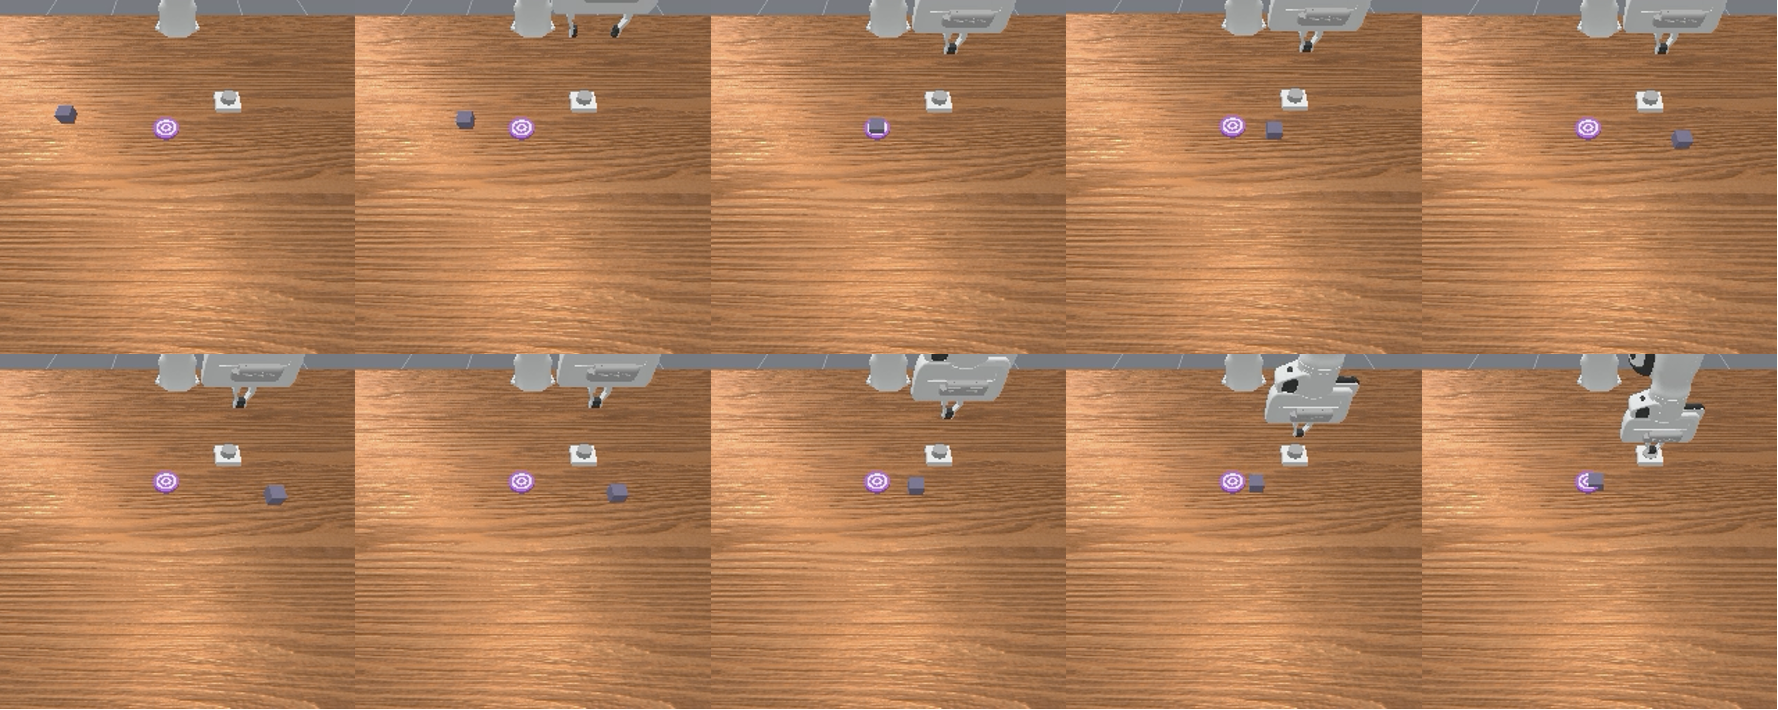
\includegraphics[width=1\linewidth]{images/tasks/stopcube.png}
    \caption{\textbf{StopCube Task Example.} In this instance, the goal is press the button to stop the cube exactly at the target on its second visit.}
    \label{fig:stopcube}
\end{figure}



\paragraph{Language Goal}
The instruction specifies the ordinal constraint ($k$-th visit) for the stop condition. e.g., ``press the button to stop the cube exactly at the target on its third visit.''

\paragraph{Task Dynamics}
The environment features a dynamic interaction phase defined by continuous movement:
\begin{enumerate}[itemsep=1pt, topsep=0pt, leftmargin=*]
    \item \textbf{Oscillating Cube:} A cube is moving back and forth between start and end positions along a straight line.
    \item \textbf{Static Behavior:} To succeed, the robot must position its end-effector over the button and remain static (hovering) until the correct timing.
    \item \textbf{Immediate Stop:}Pressing the button stops the cube instantly. The robot must press at the exact moment the cube reaches the target zone in the specified cycle, accounting for the motion delay from hover to button.
\end{enumerate}

\paragraph{Success Criteria}
\begin{itemize}[itemsep=1pt, topsep=0pt, leftmargin=*]
    \item \textbf{Precise Synchronization:} The button must be pressed strictly within the time window when the cube overlaps with the target.
    \item \textbf{Correct Ordinality:} The stop must correspond to the specified count when the cube reaches the target.
    \item \textbf{Failure:} The episode terminates early if the button is pressed too early or too late.
\end{itemize}

\clearpage


\subsection{VideoUnmask}
\label{sec:task_videounmask}

\begin{wraptable}{r}{0.5\linewidth}
    \centering
    \caption{\textit{VideoUnmask} Task Configuration.}
    \label{tab:videounmask_difficulty_config}
    \renewcommand{\arraystretch}{1.2}
    \resizebox{\linewidth}{!}{
    \begin{tabular}{l c c c}
        \toprule
        \textbf{Difficulty} & \textbf{\#Total Containers} & \textbf{\#Goal Containers} & \textbf{\#Totao Cubes} \\
        \midrule
        Easy   & 3  & 1 & 3 (red, green, blue) \\
        Medium & 5  & 1 & 3 (red, green, blue) \\
        Hard   & 10 & 2 & 3 (red, green, blue) \\
        \bottomrule
    \end{tabular}}
\end{wraptable}
The \textit{VideoUnmask} task, illustrated in Fig.~\ref{fig:videounmask}, evaluates spatial memory from a demonstration video. The robot first watches the video and infers which container hides the specified cube (red, blue, or green), then selects the corresponding container(s) during execution. Successful completion requires identifying the correct container(s) from the video and picking each required one at least once (in the specified order when multiple picks are requested), without selecting any incorrect containers.
Task configurations are summarized in Table~\ref{tab:videounmask_difficulty_config}.

\begin{figure}
    \centering
    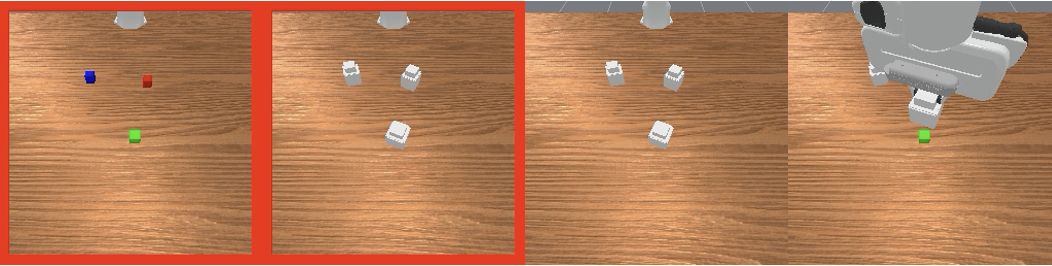
\includegraphics[width=1\linewidth]{images/tasks/videounmask.png}
    \caption{\textbf{VideoUnmask Task Example.} In this instance, after watching a video in which all cubes are masked, the robot must pick up the container hiding the green cube. Red-bordered frames denote the video-based observation prior to execution.}
    \label{fig:videounmask}
\end{figure}



\paragraph{Language Goals}
We use language instructions with increasing temporal and compositional complexity:
\begin{enumerate}[itemsep=1pt, topsep=0pt, leftmargin=*]
    \item Pick \textbf{one} container hiding a specified cube \\
    \textit{e.g., ``Watch the video carefully, then pick up the container hiding the green cube.''}
    
    \item Pick \textbf{two} containers sequentially (order matters) \\
    \textit{e.g., ``Watch the video carefully, then pick up the container hiding the green cube, and finally pick up the container hiding the red cube.''}
\end{enumerate}

\paragraph{Task Characteristics}
Each episode consists of a \textbf{video phase} followed by an \textbf{execution phase}.
\begin{itemize}[itemsep=1pt, topsep=0pt, leftmargin=*]
    \item \textbf{Video:} Multiple containers are placed on the table. Each cube (red/green/blue) is hidden under a container, and some containers may be empty. The robot remains stationary during the video.
    
    \item \textbf{Execution:} The robot must pick up the container(s) hiding the specified cube(s) described in the language instruction, using the correspondence inferred from the demonstration.
\end{itemize}

\paragraph{Success Criteria}
\begin{itemize}[itemsep=1pt, topsep=0pt, leftmargin=*]
    \item \textbf{Correct completion:} All containers hiding the specified cubes are picked up at least once, following the required order when applicable.
    
    \item \textbf{Immediate failure:} Picking any incorrect container (i.e., one hiding a non-specified cube) immediately terminates the episode.
\end{itemize}



\clearpage





\subsection{ButtonUnmask}
\label{sec:task_buttonunmask}

\begin{wraptable}{r}{0.5\linewidth}
    \centering
    \caption{\textit{ButtonUnmask} Task Configuration.}
    \label{tab:buttonunmask_difficulty_config}
    \renewcommand{\arraystretch}{1.2}
{\resizebox{\linewidth}{!}{
    \begin{tabular}{l c c c}
        \toprule
        \textbf{Difficulty} & \textbf{\#Total Containers} & \textbf{\#Goal Containers} & \textbf{\#Total Cubes} \\
        \midrule
        Easy   & 3  & 1 & 3 (red, green, blue) \\
        Medium & 5  & 1 & 3 (red, green, blue) \\
        Hard   & 15 & 2 & 3 (red, green, blue) \\
        \bottomrule
    \end{tabular}}}
\end{wraptable}
The \textit{ButtonUnmask} task, illustrated in Fig.~\ref{fig:buttonunmask}, evaluates the robot’s spatial memory for identifying hidden objects through active interaction. Unlike passive observation tasks, the robot must first press a button to reveal the scene, then determine which container hides the specified cube and pick it up.
Task configurations are given in Table~\ref{tab:buttonunmask_difficulty_config}.

\begin{figure}
    \centering
    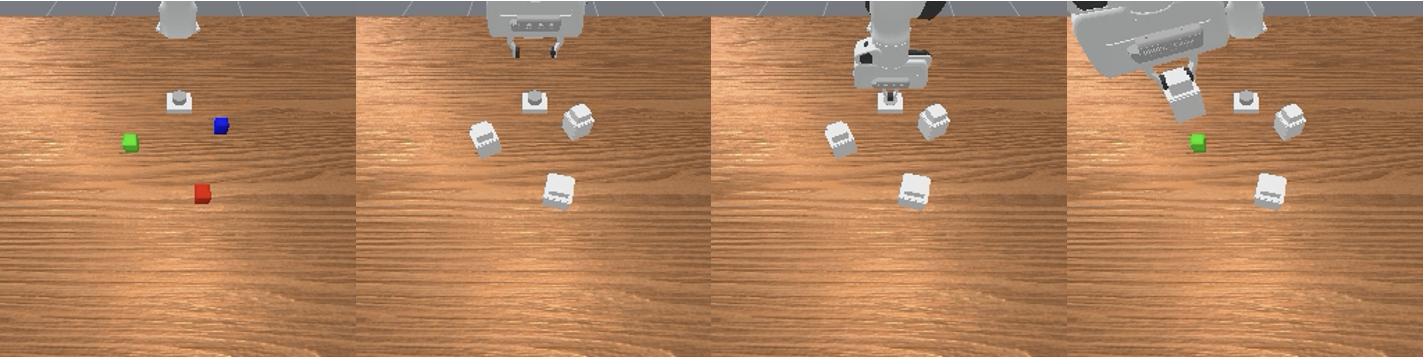
\includegraphics[width=1\linewidth]{images/tasks/buttonunmask.png}
    \caption{\textbf{ButtonUnmask Task Example.} In this instance, the robot first presses the button on the table and then selects the container hiding the green cube. During the button press, all cubes are masked.}
    \label{fig:buttonunmask}
\end{figure}



\paragraph{Language Goals}
We use language instructions with increasing compositional complexity:
\begin{enumerate}[itemsep=1pt, topsep=0pt, leftmargin=*]
    \item Pick \textbf{one} specified container by cube color \\
    \textit{e.g., ``First press the button on the table, then pick up the container hiding the green cube.''}
    
    \item Pick \textbf{two} specified containers sequentially (order matters) \\
    \textit{e.g., ``First press the button on the table, then pick up the container hiding the green cube, and finally pick up the container hiding the red cube.''}
\end{enumerate}

\paragraph{Task Characteristics}
\begin{itemize}[itemsep=1pt, topsep=0pt, leftmargin=*]
    \item \textbf{Button Pressing:} The robot need to presses the button at the beginning. During the press, multiple containers are concurrently placed on the table. Each cube is hidden under a container, and some containers may be empty. The robot needs to memorize the happening event. 
    
    \item \textbf{Unmasking:} 
    The robot identifies and picks up the container(s) hiding the specified cube(s) described in the language instruction.  When multiple pickups are required, the robot must release the first container (e.g., place it back on the table) before attempting the next.
\end{itemize}

\paragraph{Success Criteria}
\begin{itemize}[itemsep=1pt, topsep=0pt, leftmargin=*]
    \item \textbf{Correct completion:} The robot succesfully presses the button and picks up all specified containers at least once, following the required order.
    
    \item \textbf{Immediate failure:} The episode terminates early if:
    \begin{enumerate}[itemsep=1pt, topsep=0pt, leftmargin=*]
        \item The robot picks up any container before completing the button-press phase.
        \item The robot picks up an incorrect container (i.e., one hiding a non-specified cube).
    \end{enumerate}
\end{itemize}



\clearpage



\subsection{VideoUnmaskSwap}
\label{sec:task_videounmaskswap}

\begin{wraptable}{r}{0.6\linewidth}
    \centering
    \caption{\textit{VideoUnmaskSwap} Task Configuration.}
    \label{tab:videounmaskswap_difficulty_config}
    \renewcommand{\arraystretch}{1.2}
    \resizebox{\linewidth}{!}{
    \begin{tabular}{l c c c c}
        \toprule
        \textbf{Difficulty} & \textbf{\#Total Containers} & \textbf{\#Swap Times} & \textbf{\#Goal Containers} & \textbf{\#Total Cubes} \\
        \midrule
        Easy   & 3 & 1--2 & 1--2 & 3 (red, green, blue) \\
        Medium & 4 & 1--2 & 1 & 3 (red, green, blue) \\
        Hard   & 4 & 2--3 & 2 & 3 (red, green, blue) \\
        \bottomrule
    \end{tabular}}
    % \vspace{-0.5cm}
\end{wraptable}
The \textit{VideoUnmaskSwap} task (Fig.~\ref{fig:videounmaskswap}) evaluates spatial memory from a video demonstration. The robot observes containers swapping positions, tracks the correct containers, and then retrieves them during execution.
Task configurations are summarized in Table~\ref{tab:videounmaskswap_difficulty_config}.

\begin{figure}
    \centering
    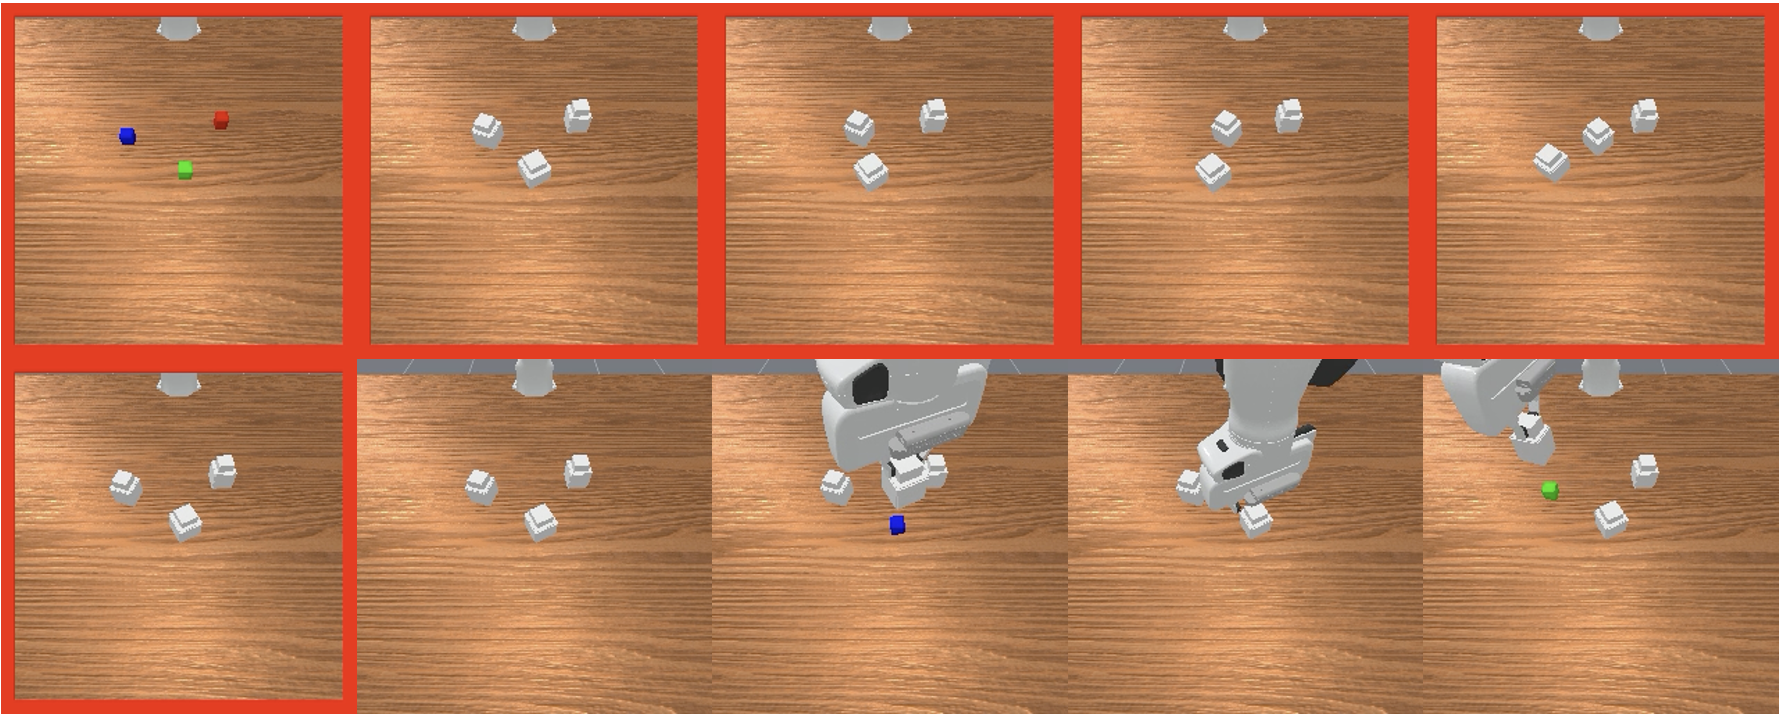
\includegraphics[width=1\linewidth]{images/tasks/videounmaskswap.png}
    \caption{\textbf{VideoUnmaskSwap Task Example.} In this instance, the robot first watches the video, then picks up the container hiding the blue cube, followed by the one hiding the green cube. The video shows that all cubes are being masked by containers,  with some containers swapped between locations. Red-bordered frames denote the video-based initial observations provided before execution.
}
    \label{fig:videounmaskswap}
\end{figure}
\paragraph{Language Goals}
We use language instructions with increasing temporal and compositional complexity:
\begin{enumerate}[itemsep=1pt, topsep=0pt, leftmargin=*]
    \item Pick \textbf{one} specified container \\
    \textit{e.g., ``Watch the video carefully, then pick up the container hiding the blue cube.''}
    
    \item Pick \textbf{two} specified containers sequentially (order matters) \\
    \textit{e.g., ``Watch the video carefully, then pick up the container hiding the blue cube, and finally pick up the container hiding the red cube.''}
\end{enumerate}

\paragraph{Task Characteristics}
Each episode consists of a \textbf{video phase} followed by an \textbf{execution phase}.
\begin{itemize}[itemsep=1pt, topsep=0pt, leftmargin=*]
    \item \textbf{Video:} Multiple containers are placed on the table. Each cube (red/green/blue) is hidden under a container, and some containers may be empty. The robot remains stationary while the containers swap positions multiple times according to the difficulty setting.
    
    \item \textbf{Execution:} The robot must pick up the container(s) hiding the specified cube(s) described in the language instruction, tracking each container’s identity across the observed swaps.
\end{itemize}

\paragraph{Success Criteria}
\begin{itemize}[itemsep=1pt, topsep=0pt, leftmargin=*]
    \item \textbf{Correct completion:} All specified containers are picked up at least once, following the required order when applicable.
    
    \item \textbf{Immediate failure:} Picking any incorrect container (i.e., one hiding a non-specified cube) immediately terminates the episode.
\end{itemize}



\clearpage







\subsection{ButtonUnmaskSwap}
\label{sec:task_buttonunmaskswap}

\begin{wraptable}{r}{0.5\linewidth}
    \centering
    \caption{\textit{ButtonUnmaskSwap} Task Configuration.}
    \label{tab:buttonunmaskswap_difficulty_config}
    \renewcommand{\arraystretch}{1.2}
    \resizebox{\linewidth}{!}{
    \begin{tabular}{l c c c c}
        \toprule
        \textbf{Difficulty} & \textbf{\#Total Containers} & \textbf{\#Goal Containers} & \textbf{\#Swap Times} & \textbf{\#Total Cubes} \\
        \midrule
        Easy   & 3 & 1--2 & 1--2 & 3 (red, green, blue) \\
        Medium & 4 & 1    & 1--2 & 3 (red, green, blue) \\
        Hard   & 4 & 2    & 2--3 & 3 (red, green, blue) \\
        \bottomrule
    \end{tabular}}
\end{wraptable}
The \textit{ButtonUnmaskSwap} task (Fig.~\ref{fig:buttonunmaskswap}) evaluates spatial memory under active interaction. The robot must press both buttons during container hiding and swapping, track the container concealing the target cube, and finally lift the correct one.
Task configurations are summarized in Table~\ref{tab:buttonunmaskswap_difficulty_config}.

\begin{figure}
    \centering
    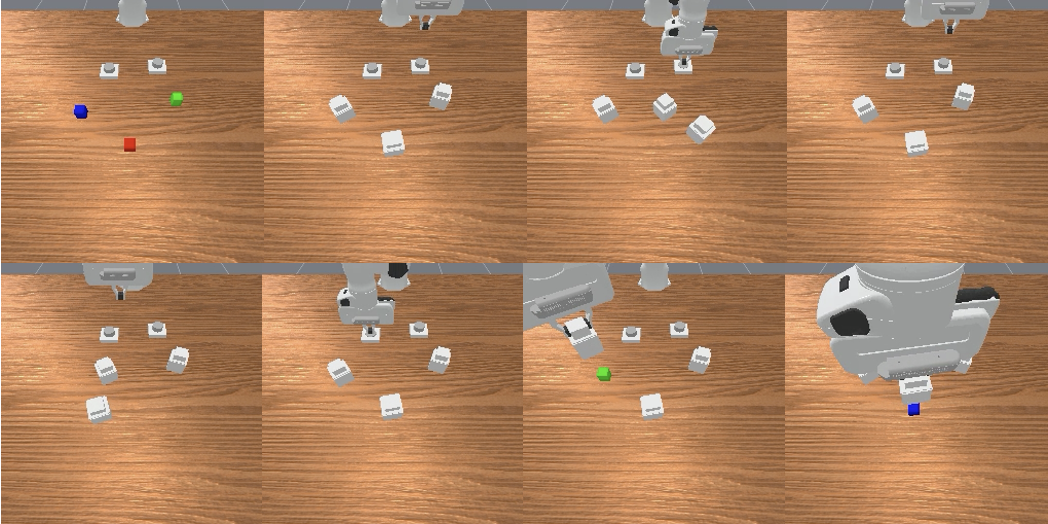
\includegraphics[width=0.85\linewidth]{images/tasks/buttonunmaskswap.png}
    \caption{\textbf{ButtonUnmaskSwap Task Example.} In this instance, the robot first presses both buttons on the table, then picks up the container hiding the green cube, followed by the one hiding the blue cube. During the button presses, all cubes are masked and their locations are swapped.}
    \label{fig:buttonunmaskswap}
\end{figure}
\paragraph{Language Goals}
We use language instructions with increasing complexity:
\begin{enumerate}[itemsep=1pt, topsep=0pt, leftmargin=*]
    \item Pick \textbf{one} specified container \\
    \textit{e.g., ``First press both buttons on the table, then pick up the container hiding the red cube.''}
    
    \item Pick \textbf{two} specified containers sequentially (order matters) \\
    \textit{e.g., ``First press both buttons on the table, then pick up the container hiding the green cube, and finally pick up the container hiding the red cube.''}
\end{enumerate}
\paragraph{Task Characteristics}
\begin{itemize}[itemsep=1pt, topsep=0pt, leftmargin=*]
    \item \textbf{Button Pressing:} The robot needs to press both buttons. During the pressing, multiple containers are placed on the table to enclose the cubes, after which the some containers swap positions. 
    
    \item \textbf{Unmasking:} The robot must pick up the container(s) hiding the specified cube color(s) described in the language instruction, following the same order when multiple pickups are required.
\end{itemize}
\paragraph{Success Criteria}
\begin{itemize}[itemsep=1pt, topsep=0pt, leftmargin=*]
    \item \textbf{Correct completion:} The robot presses both buttons and picks up all specified containers at least once, following the required order.
    
    \item \textbf{Immediate failure:} The episode terminates early if:
    \begin{enumerate}[itemsep=1pt, topsep=0pt, leftmargin=*]
        \item The robot picks up any container before completing the button-press phase.
        \item The robot picks up an incorrect container (i.e., one hiding a non-specified cube).
    \end{enumerate}
\end{itemize}

\clearpage




\subsection{PickHighlight}
\label{sec:task_pickhighlight}

\begin{wraptable}{r}{0.35\linewidth}
    \centering
    \caption{\textit{PickHighlight} Task Configuration.}
    \label{tab:pickhighlight_difficulty_config}
    \renewcommand{\arraystretch}{1.2}
{\resizebox{\linewidth}{!}{
    \begin{tabular}{l c c}
        \toprule
        \textbf{Difficulty} & \textbf{\#Total Cubes} & \textbf{\#Goal Cubes} \\
        \midrule
        Easy   & 3 & 1 \\
        Medium & 4 & 2 \\
        Hard   & 6 (cluster) & 3 \\
        \bottomrule
    \end{tabular}}}
\end{wraptable}
The \textit{PickHighlight} task, shown in Fig.~\ref{fig:pickhighlight}, evaluates the robot’s short-term object memory. The robot must press a button to briefly highlight specific cubes, memorize the highlighted cubes, and then pick them up after the cues disappear. This tests the robot’s ability to maintain a working memory of transient object states. Detailed Task Configurations are summarized in Table~\ref{tab:pickhighlight_difficulty_config}.

\begin{figure}
    \centering
    
    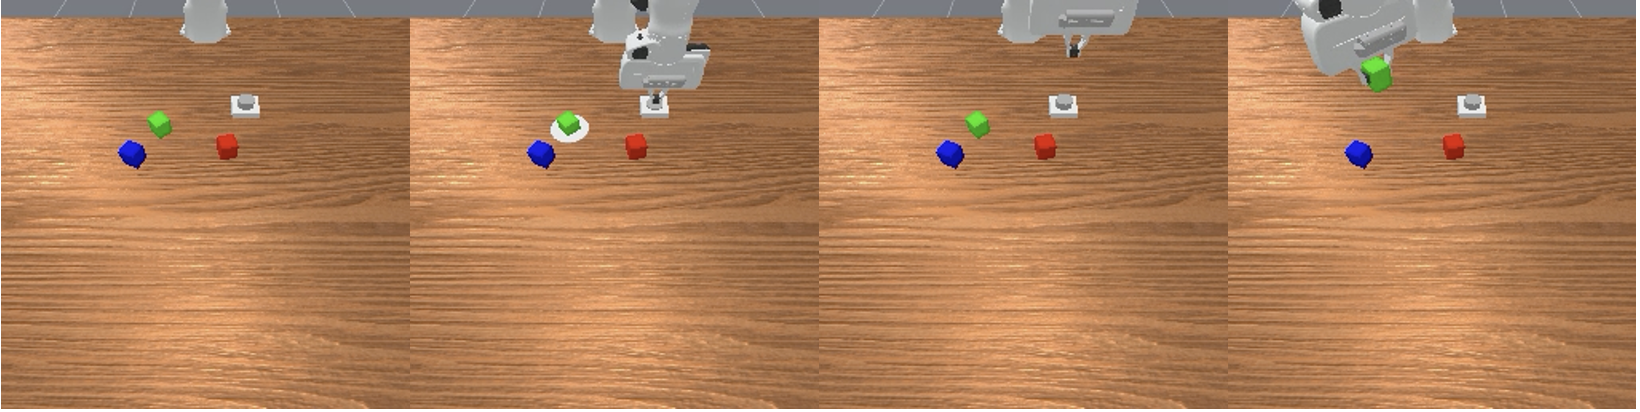
\includegraphics[width=1\linewidth]{images/tasks/pickhighlight.png}
    \caption{\textbf{PickHighlight Task Example.} In this instance, the goal is first press the button, then pick up all cubes \textit{highlighted by white area}, finally press the button again to stop. During the button pressing, the green cube was highlighted with a white area on the table, the robot needs to capture this information, and pick up the correct cubes.}
    \label{fig:pickhighlight}
\end{figure}



\paragraph{Language Goals}
The task involves a multi-stage sequential command: Press button, memorize, and pick highlighted objects. \\
    \textit{e.g., ``first press the button, then pick up all highlighted cubes, finally press the button again to stop.''}

\paragraph{Task Characteristics}
\begin{itemize}[itemsep=1pt, topsep=0pt, leftmargin=*]
    \item \textbf{Button Pressing:} The robot must first press the button. During the press, the specified cubes are briefly highlighted with a white visual indicator for a fixed number of timesteps.
    
    \item \textbf{Highlighted Cube Picking:} The robot must identify and pick up all cubes highlighted during this window. If multiple cubes are specified, each must be picked up at least once.
\end{itemize}

\paragraph{Success Criteria}
\begin{itemize}[itemsep=1pt, topsep=0pt, leftmargin=*]
    \item \textbf{Correct completion:} The robot successfully presses the button  and picks up all correct cubes at least once.
\item \textbf{Immediate failure:} The episode terminates early if:
    \begin{enumerate}[itemsep=1pt, topsep=0pt, leftmargin=*]
        \item The robot fails to press the button before attempting a pick.
        \item The robot picks up any wrong cubes (i.e., a cube that was not highlighted).
    \end{enumerate}
\end{itemize}
\clearpage




\subsection{VideoRepick}
\label{sec:task_videorepick}

\begin{wraptable}{r}{0.5\linewidth}
    \centering
    \caption{\textit{VideoRepick} Task Configuration.}
    \label{tab:videorepick_difficulty_config}
    \renewcommand{\arraystretch}{1.2}
    \resizebox{1\linewidth}{!}{
    \begin{tabular}{l c c c}
        \toprule
        \textbf{Difficulty} & \textbf{\#Cubes} & \textbf{\#Swap Times} & \textbf{\#Repeatition} \\
        \midrule
        Easy   & 3 (same color)            & 1--2 & 1--3 \\
        Medium & 3 (same color)            & 2--3 & 1--3 \\
        Hard   & 15 (different colors, clutter scene)     & 0 & 1--3 \\
        \bottomrule
    \end{tabular}}
\end{wraptable}
The \textit{VideoRepick} task is illustrated in Fig.~\ref{fig:videorepick}. The robot must watch a demonstration video to identify a specific cube instance, locate the same instance in the current scene (even if the cubes have moved or swapped), and repeat the pick-and-place action exactly $N$ times before pressing a stop button. Task configurations are provided in Table~\ref{tab:videorepick_difficulty_config}.

\begin{figure}
    \centering
    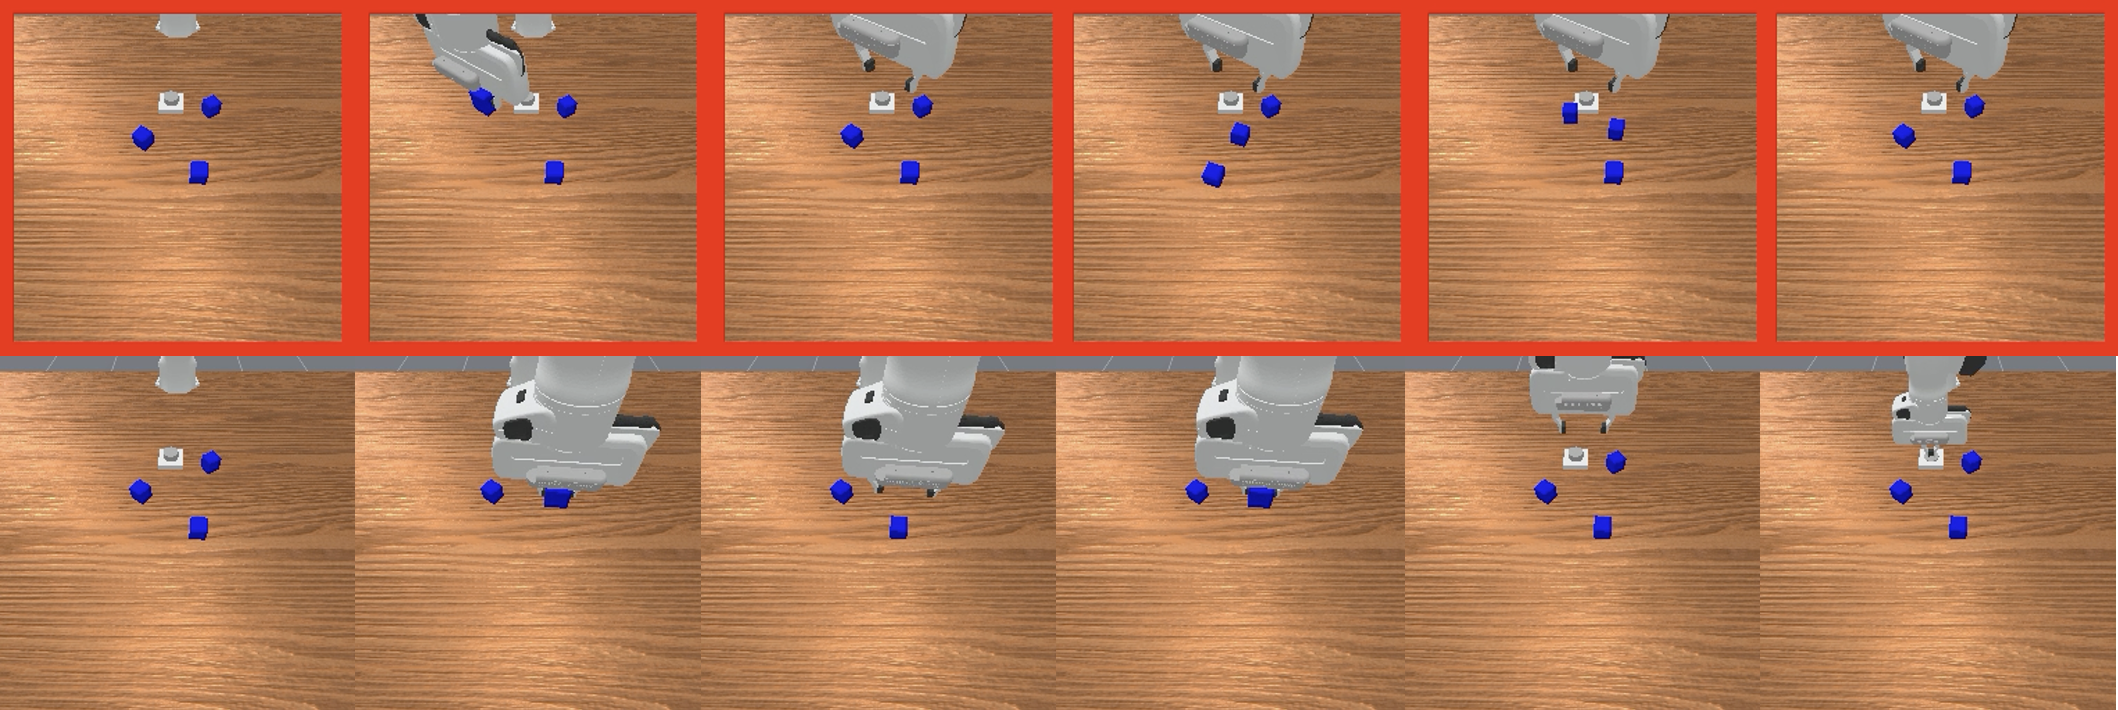
\includegraphics[width=1\linewidth]{images/tasks/videorepick.png}
    \caption{\textbf{VideoRepick Task Example.} In this instance, the robot first watches a video, then picks up the same previously picked cube twice, and finally presses the button to stop. Red-bordered frames denote the video-based observations shown prior to execution.}
    \label{fig:videorepick}
\end{figure}


\paragraph{Language Goals}
\begin{itemize}[itemsep=1pt, topsep=0pt, leftmargin=*]
\item Repeat picking the cube for $N$ times that was previously picked in the video, then stop.\\
\textit{e.g., ``Watch the video carefully, then pick up the same cube that was previously picked twice, and finally press the button to stop.''}
\end{itemize}

\paragraph{Task Characteristics}
Each episode consists of a \textbf{video phase} and an \textbf{execution phase}.
\begin{itemize}[itemsep=1pt, topsep=0pt, leftmargin=*]
\item \textbf{Video:} the robot picks up a specified cube and places it. Afterward, the robot remains still while the cubes may swap positions, requiring the agent to track the correct cube from the video.
\item \textbf{Execution:} the robot locates the same previously picked cube and repeats the pick-and-place action for a specific number of cycles specified in the instruction.
\end{itemize}

\paragraph{Success Criteria}
\begin{itemize}[itemsep=1pt, topsep=0pt, leftmargin=*]
\item \textbf{Correct completion:} complete exactly $N$ pick-and-place repetitions with the demonstrated cube, then press the button.
\item \textbf{Immediate failure:} the episode terminates early if:
\begin{enumerate}[itemsep=1pt, topsep=0pt, leftmargin=*]
\item the robot picks up the wrong cube,
\item the button is pressed before finishing $N$ repetitions, or
\item the robot completes more than $N$ repetitions.
\end{enumerate}
\end{itemize}

\clearpage


\subsection{VideoPlaceButton}
\label{sec:task_videoplacebutton}

\begin{wraptable}{r}{0.35\linewidth}
    \centering
    \caption{\textit{VideoPlaceButton} Task Configuration.}
    \label{tab:videoplacebutton_difficulty_config}
    \renewcommand{\arraystretch}{1.2}
    {\resizebox{\linewidth}{!}{
    \begin{tabular}{l c c c}
        \toprule
        \textbf{Difficulty} & \textbf{\#Cubes} & \textbf{\#Targets} & \textbf{Target Swapping} \\
        \midrule
        Easy   & 1  & 3 & No \\
        Medium & 3  & 4 & No \\
        Hard   & 3  & 4 & Yes \\
        \bottomrule
    \end{tabular}}}
\end{wraptable}

The \textit{VideoPlaceButton} task, illustrated in Fig.~\ref{fig:videoplacebutton}, tests long-video temporal reasoning and object grounding. The robot must watch a long video in which a cube is placed on multiple targets, separated by a distinct button press, and then parse a natural language instruction specifying a temporal relation (e.g., \textit{before} or \textit{after} the button press) to identify the correct destination. Task configurations are summarized in Table~\ref{tab:videoplacebutton_difficulty_config}.

\begin{figure}
    \centering
    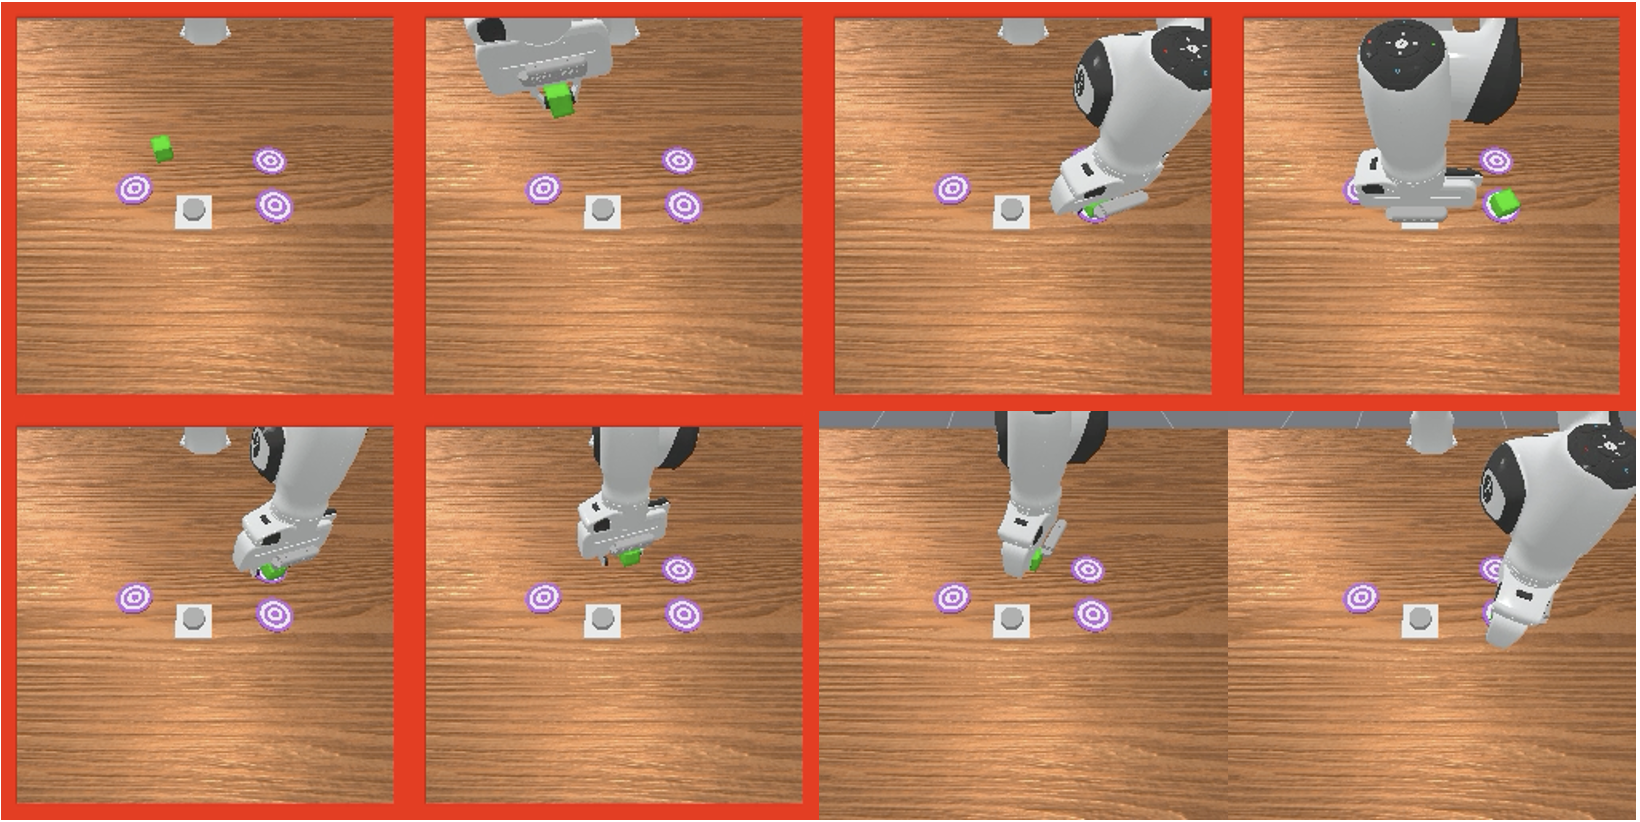
\includegraphics[width=0.9\linewidth]{images/tasks/videoplacebutton.png}
    \caption{\textbf{VideoPlaceButton Task Example.} In this example, the robot first observes a video depicting an interleaved sequence of cube placements and button presses, and then places the cube onto the correct target corresponding to its location prior to the button press. Red-bordered frames indicate the video-based observations provided before execution. }
    \label{fig:videoplacebutton}
\end{figure}




\paragraph{Language Goals}
We use language instruction to specify a cube and the target location relative to the button press event (\textit{before/after}): \textit{e.g., ``Watch the video carefully and place the blue cube on the target where it was placed immediately before the button was pressed.''}

\paragraph{Task Characteristics}
Each episode has a \textbf{video phase} and an \textbf{execution phase}.
\begin{itemize}[itemsep=1pt, topsep=0pt, leftmargin=*]
    \item \textbf{Video:} the robot picks up a cube and alternates between placing it on different targets and pressing a button. In the \textit{Hard} mode, two targets swap positions after the sequence finishes.
    \item \textbf{Execution:} the robot must identify the correct cube , pick it up, and place it on the correct target according to the specified temporal relation (e.g., before or after the button press).
\end{itemize}


\paragraph{Success Criteria}
\begin{itemize}[itemsep=1pt, topsep=0pt, leftmargin=*]
    \item \textbf{Correct completion:} successfully pick the correct color cube and placing it on the correct target.
\item \textbf{Immediate failure:} The episode terminates early if: (1) pick a wrong cube; (2) place the cube on the wrong target.
\end{itemize}

\clearpage



\subsection{VideoPlaceOrder}
\label{sec:task_videoplaceorder}

\begin{wraptable}{r}{0.35\linewidth}
    \centering
    \caption{\textit{VideoPlaceOrder} Task Configuration.}
    \label{tab:videoplaceorder_difficulty_config}
    \renewcommand{\arraystretch}{1.2}
   {\resizebox{\linewidth}{!}{
    \begin{tabular}{l c c c}
        \toprule
        \textbf{Difficulty} & \textbf{\#Cubes} & \textbf{\#Targets} & \textbf{Target Swapping} \\
        \midrule
        Easy   & 1 & 4 & No \\
        Medium & 3 & 4 & No \\
        Hard   & 3 & 4 & Yes\\
        \bottomrule
    \end{tabular}}}
\end{wraptable}

The \textit{VideoPlaceOrder} task, illustrated in Fig.~\ref{fig:videoplaceorder}, evaluates long-video temporal reasoning and object grounding. The robot must watch a long video to memorize the sequence of cube placements, then parse a natural language instruction specifying an ordinal position (e.g., ``the third target'') to identify the correct destination.
Task configurations are summarized in Table~\ref{tab:videoplaceorder_difficulty_config}.

\begin{figure}
    \centering
    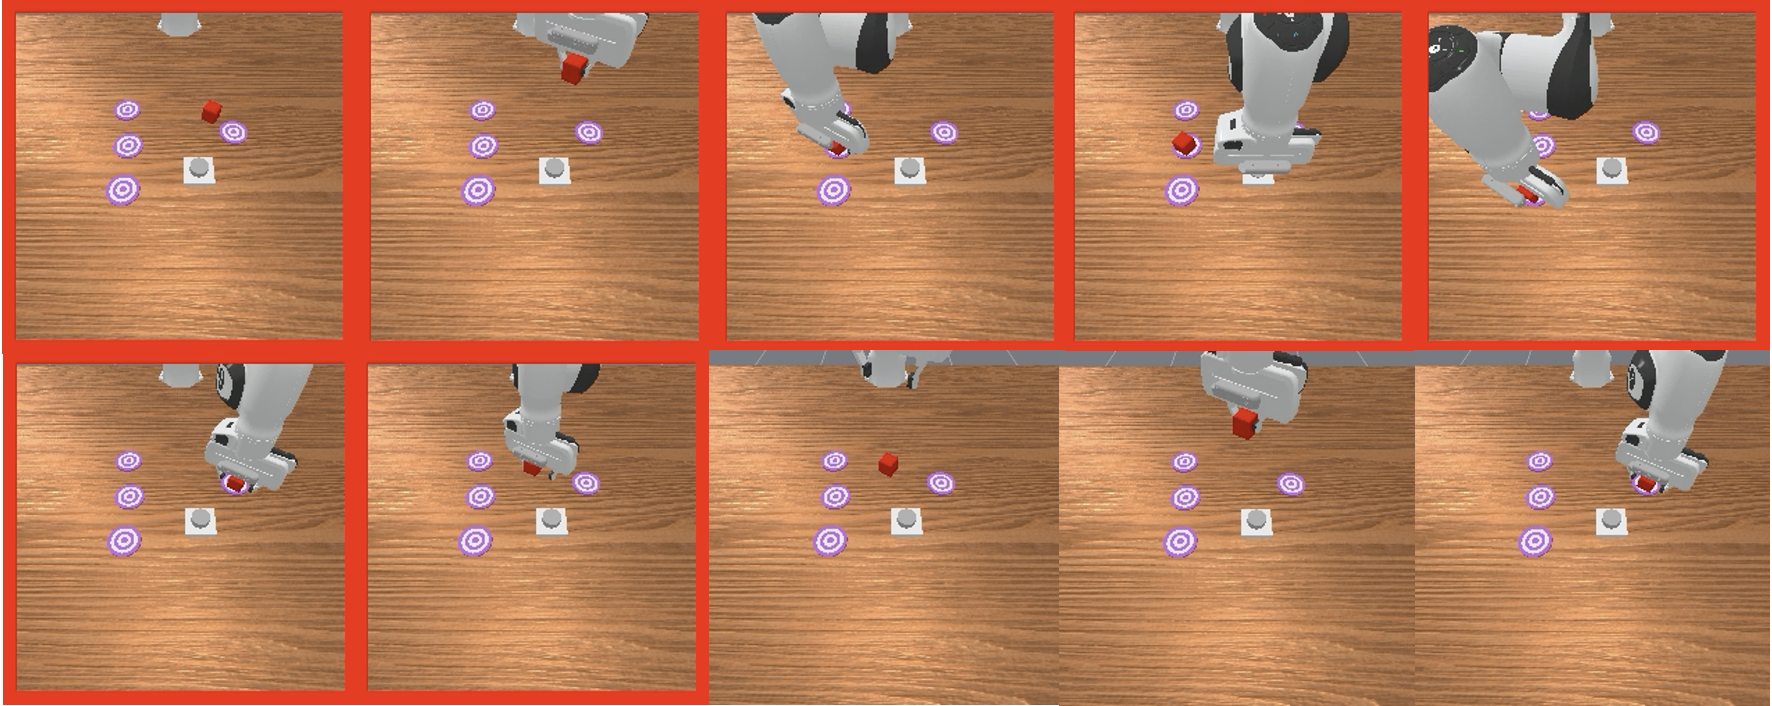
\includegraphics[width=1\linewidth]{images/tasks/videoplaceorder.png}
    \caption{\textbf{VideoPlaceOrder Task Example.} In this instance, the goal is to place the red cube on the \textit{third} target where it was previously placed in the given video. Red-bordered frames denote the video-based observation prior to execution. }
    \label{fig:videoplaceorder}
\end{figure}


\paragraph{Language Goals}
We use language instructions that specify the cube and the ordinal rank of the target location relative to the video history, \textit{e.g., ``Watch the video carefully and place the red cube on the third target where it was placed.''}

\paragraph{Task Characteristics}
Each episode consists of a \textbf{video phase} and an \textbf{execution phase}.
\begin{itemize}[itemsep=1pt, topsep=0pt, leftmargin=*]
\item \textbf{Video:} the robot picks up a cube and places it onto multiple targets in a specific sequence, pressing a button between placements. In the \textit{Hard} mode, two targets swap positions after the sequence finishes.
\item \textbf{Execution:} the robot identifies and picks up the correct cube, then places it onto the correct target corresponding to the requested ordinal rank (e.g., the third target visited).
\end{itemize}

\paragraph{Success Criteria}
\begin{itemize}[itemsep=1pt, topsep=0pt, leftmargin=*]
\item \textbf{Correct completion:} successfully pick up the correct colored cube and place it on the target indicated by the specified temporal order.
\item \textbf{Immediate failure:} the episode terminates early if: (1) the robot picks up the wrong cube; or (2) the cube is placed on the wrong target.
\end{itemize}

\clearpage



\subsection{MoveCube}
\label{sec:task_movecube}

The \textit{MoveCube} task, illustrated in Fig.~\ref{fig:movecube}, assesses the robot's ability to recognize and reproduce distinct action semantics. The task requires the robot to observe a video demonstration where a cube is moved to a target using one of three specific manipulation manners: (1) hooking it with a tool; (2) pushing it with a closed gripper; or (3) performing a standard pick-and-place operation. Success requires correctly inferring the underlying motion strategy from videos and executing the exact same method during the execution phase.

\begin{figure}
    \centering
    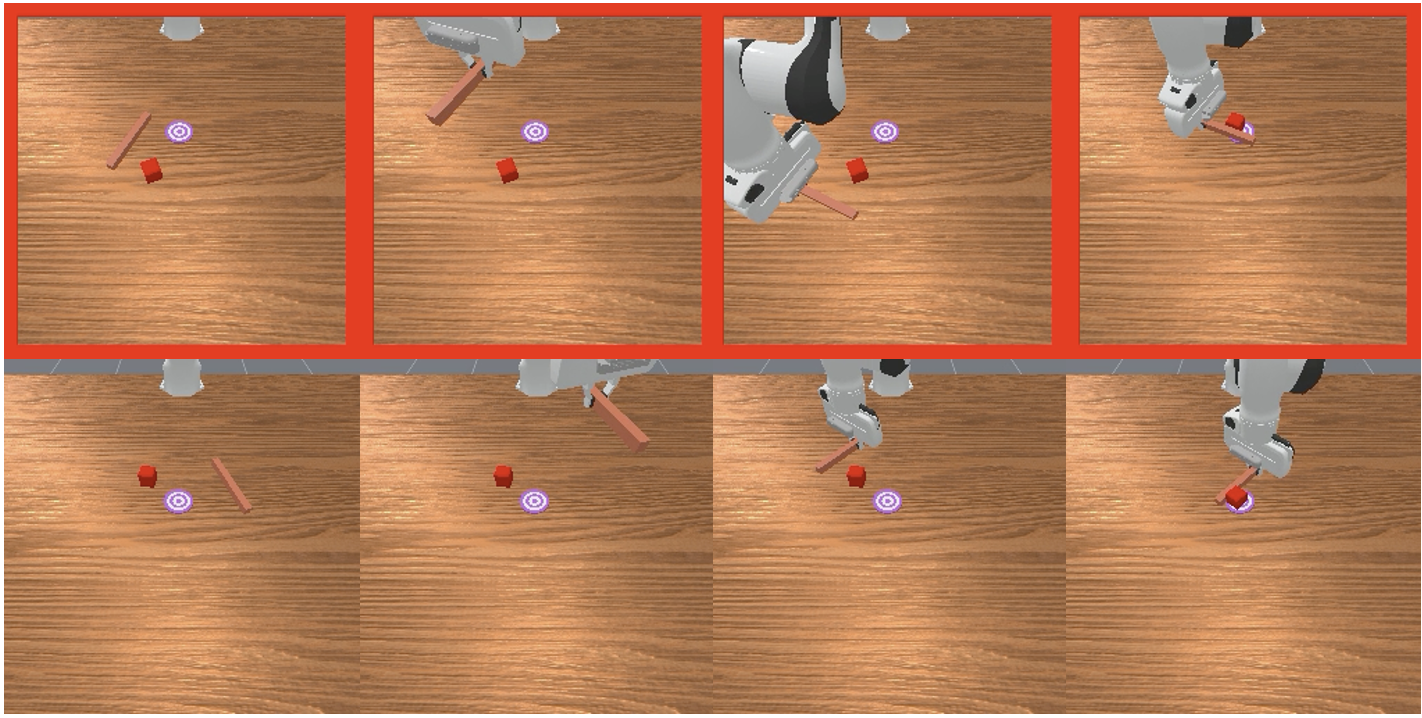
\includegraphics[width=0.85\linewidth]{images/tasks/movecube.png}
    \caption{\textbf{MoveCube Task Example.} In this instance, the robot must watch the video carefully, then move the cube to the target in the same manner as demonstrated. Red-bordered frames denote the video-based observation prior to execution. }
    \label{fig:movecube}
\end{figure}

\paragraph{Language Goal} \textit{``Watch the video carefully, then move the cube to the target in the same manner as before.''}
\paragraph{Task Characteristics}
Each episode has a \textbf{video phase} and an \textbf{execution phase}.

\begin{itemize}[itemsep=1pt, topsep=0pt, leftmargin=*]
\item \textbf{Video:} The robot moves a cube to a target location using one of three manipulation methods:
\begin{enumerate}[itemsep=1pt, topsep=0pt, leftmargin=*]
\item \textbf{Hooking:} pick up a peg tool and using it to hook the cube to the target.
\item \textbf{Pushing:} close the gripper and use the gripper to push the cube across the surface to the target.
\item \textbf{Pick-and-Place:} grasp the cube directly, lifting it, and placing it on the target.
\end{enumerate}
\item \textbf{Execution:} After the demonstration, the cube and target are reset to \textit{new random positions}. The robot must identify the method used in the video demonstration and replicate it exactly, adapting it to the new  configuration.
\end{itemize}

\paragraph{Success Criteria}
\begin{itemize}[itemsep=1pt, topsep=0pt, leftmargin=*]
\item \textbf{Correct completion:} The robot successfully moves the cube to the target using the same manipulation primitive observed in the demonstration.
\item \textbf{Immediate failure:} The episode terminates immediately if the robot attempts a different method than the one demonstrated (e.g., picking up the cube when a push was demonstrated, or using the tool when a direct grasp was demonstrated).
\end{itemize}
\clearpage




\subsection{InsertPeg}
\label{sec:task_insertpeg}

The \textit{InsertPeg} task, illustrated in Fig.~\ref{fig:insertpeg}, evaluates fine-grained visual perception and procedural/object memory. The robot observes a demonstration to determine which peg to select, which end to grasp, and which side to insert, then reproduces the same manipulation after the scene is reset to the same initial configuration as in the video. 
% Success requires maintaining object and pose correspondence to re-identify the correct peg and replicate the demonstrated strategy.

\begin{figure}
    \centering
    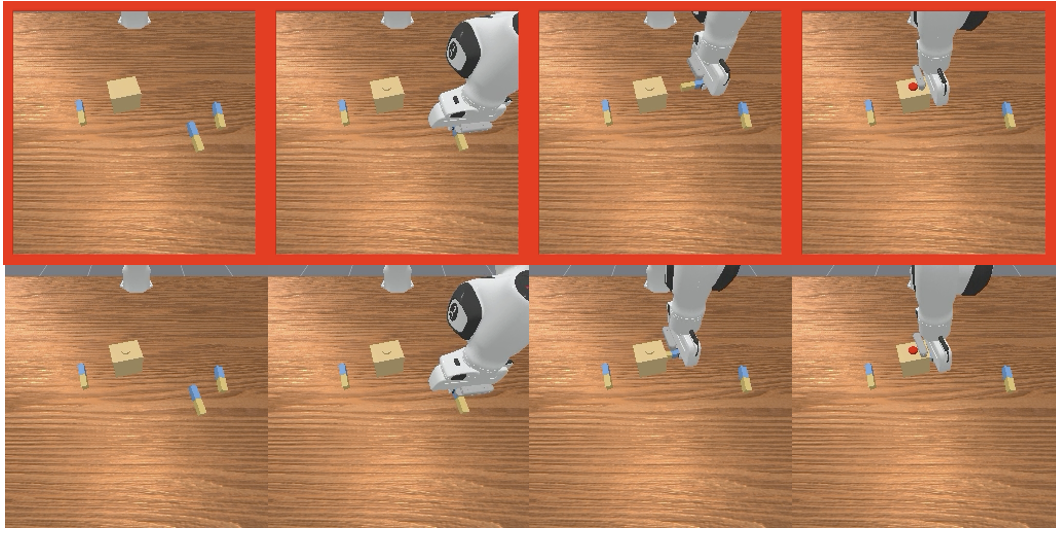
\includegraphics[width=0.85\linewidth]{images/tasks/insertpeg.png}
    \caption{\textbf{InsertPeg Task Example.}  In this instance, the robot must watch the video carefully, then grasp the same peg at the same end and insert it into the same side of the box as demonstrated.  Red-bordered frames denote the video-based observation prior to execution. }
    \label{fig:insertpeg}
\end{figure}

\paragraph{Language Goal} \textit{``Watch the video carefully, then grasp the same peg at the same end and insert it into the same side of the box as in the video.''}

\paragraph{Task Characteristics}
Each episode consists of a \textbf{video phase} and an \textbf{execution phase}.
\begin{itemize}[itemsep=1pt, topsep=0pt, leftmargin=*]
    \item \textbf{Video:} The robot picks up a peg by grasping a specific end (head or tail) and inserts it into the box from a specific side (left or right). After the demonstration, all pegs are reset to their original positions and orientations without randomness.
    \item \textbf{Execution:} The robot must identify the correct peg based on video demonstrations, then grasp the correct peg at the same end and insert it into the box from the demonstrated side.
\end{itemize}

\paragraph{Success Criteria}
\begin{itemize}[itemsep=1pt, topsep=0pt, leftmargin=*]
    \item \textbf{Correct completion:} The robot grasps the correct peg by the correct end and inserts it into the box from the correct side.
    \item \textbf{Immediate failure:} The episode terminates early if:
    \begin{enumerate}
        \item The robot picks up an incorrect peg.
        \item The robot grasps the wrong end of the peg (e.g., grasping the head when the tail was demonstrated, or vice versa).
        \item The robot inserts the peg from the wrong side of the box (e.g., inserting from the left when the right side was demonstrated).
    \end{enumerate}
\end{itemize}

\clearpage






\subsection{PatternLock}
\label{sec:task_patternlock}

\begin{wraptable}{r}{0.35\linewidth}
    \centering
    \caption{\textit{PatternLock} Task Configuration}
    \label{tab:patternlock_difficulty_config}
    \renewcommand{\arraystretch}{1.2}
    \resizebox{0.8\linewidth}{!}{
    \begin{tabular}{@{} l c c @{}}
        \toprule
        \textbf{Difficulty} & \textbf{Grid Size} & \textbf{Pattern Length} \\
        \midrule
        \textbf{Easy}   & 3$\times$3  & 2--4 \\
        \textbf{Medium} & 4$\times$4  & 3--5 \\
        \textbf{Hard}   & 5$\times$5  & 4--8 \\
        \bottomrule
    \end{tabular}}
\end{wraptable}

The \textit{PatternLock} task, illustrated in Fig.~\ref{fig:patternlock}, evaluates the robot’s long-horizon procedural memory from a video demonstration. The robot observes a stick attached to the end-effector tracing a continuous pattern over a NxN grid of gray targets, and must then reproduce the same trajectory during execution.
Success requires following the full demonstrated sequence without skipping or moving to incorrect targets.
\begin{figure}
    \centering
    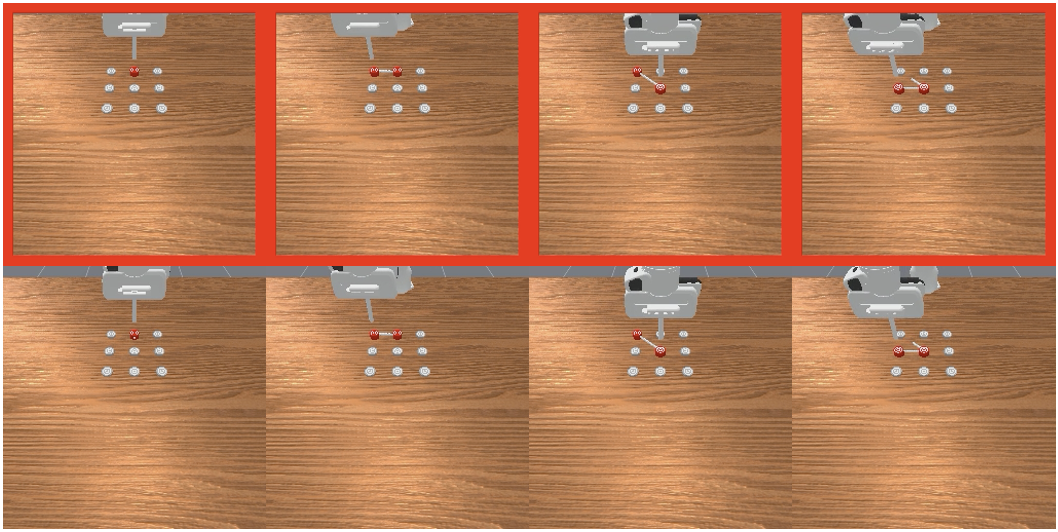
\includegraphics[width=0.85\linewidth]{images/tasks/patternlock.png}
    \caption{\textbf{PatternLock Task Example.} In this instance, the goal is to watch the video carefully and then use the stick attached to the robot to retrace the same pattern shown in the video. Red-bordered frames denote the video-based observations prior to execution.}
    \label{fig:patternlock}
\end{figure}




\paragraph{Language Goal} \textit{``Watch the video carefully, then use the stick attached to the robot to retrace the same pattern shown in the video.''}

\paragraph{Task Characteristics}

Each episode consists of a \textbf{video phase} and an \textbf{execution phase}.

\begin{itemize}[itemsep=1pt, topsep=0pt, leftmargin=*]

\item \textbf{Demonstration:} The robot uses a stick to trace a continuous pattern over a target grid, defining an ordered sequence of targets.

\item \textbf{Execution:} After reset, the robot must move the gripper to retrace the targets in the same order continually. The environment provides real-time feedback during tracing:
\begin{itemize}[itemsep=1pt, topsep=0pt, leftmargin=*]
    \item \textbf{Target highlighting feedback:} A gray target turns red when the stick is near to it, indicating a valid visit.
    \item \textbf{Trajectory trace feedback:} A line renders the stick-tip trajectory in real time.

\end{itemize}


\end{itemize}

\paragraph{Success Criteria}

\begin{itemize}[itemsep=1pt, topsep=0pt, leftmargin=*]

\item \textbf{Correct completion:} The robot visits all targets in the correct order following demonstration.

\item \textbf{Immediate failure:} the episode terminates early if the robot deviates from the demonstrated order.

\end{itemize}


\clearpage


\subsection{RouteStick}
\label{sec:task_routestick}

\begin{wraptable}{r}{0.35\linewidth}
    \centering
    \caption{RouteStick Task Configuration}
    \label{tab:routestick_difficulty_config}
    \renewcommand{\arraystretch}{1.2}
    \resizebox{0.8\linewidth}{!}{
    \begin{tabular}{@{} l c c @{}}
        \toprule
        \textbf{Difficulty} & \textbf{Path Length} & \textbf{Backtracking} \\
        \midrule
        \textbf{Easy}   & 2--3  & No \\
        \textbf{Medium} & 4--5  & No \\
        \textbf{Hard}   & 4--7  & Yes \\
        \bottomrule
    \end{tabular}}
\end{wraptable}


The \textit{RouteStick} task, illustrated in Fig.~\ref{fig:routestick}, evaluates long-horizon, geometry-aware procedural memory from a video demonstration. The robot observes a demonstration in which a stick attached to the end-effector navigates through a field of fixed vertical obstacles while visiting a sequence of targets. Successful completion requires circling each obstacle in the demonstrated direction (clockwise or counterclockwise) and following a single continuous trajectory.


\begin{figure}
    \centering
    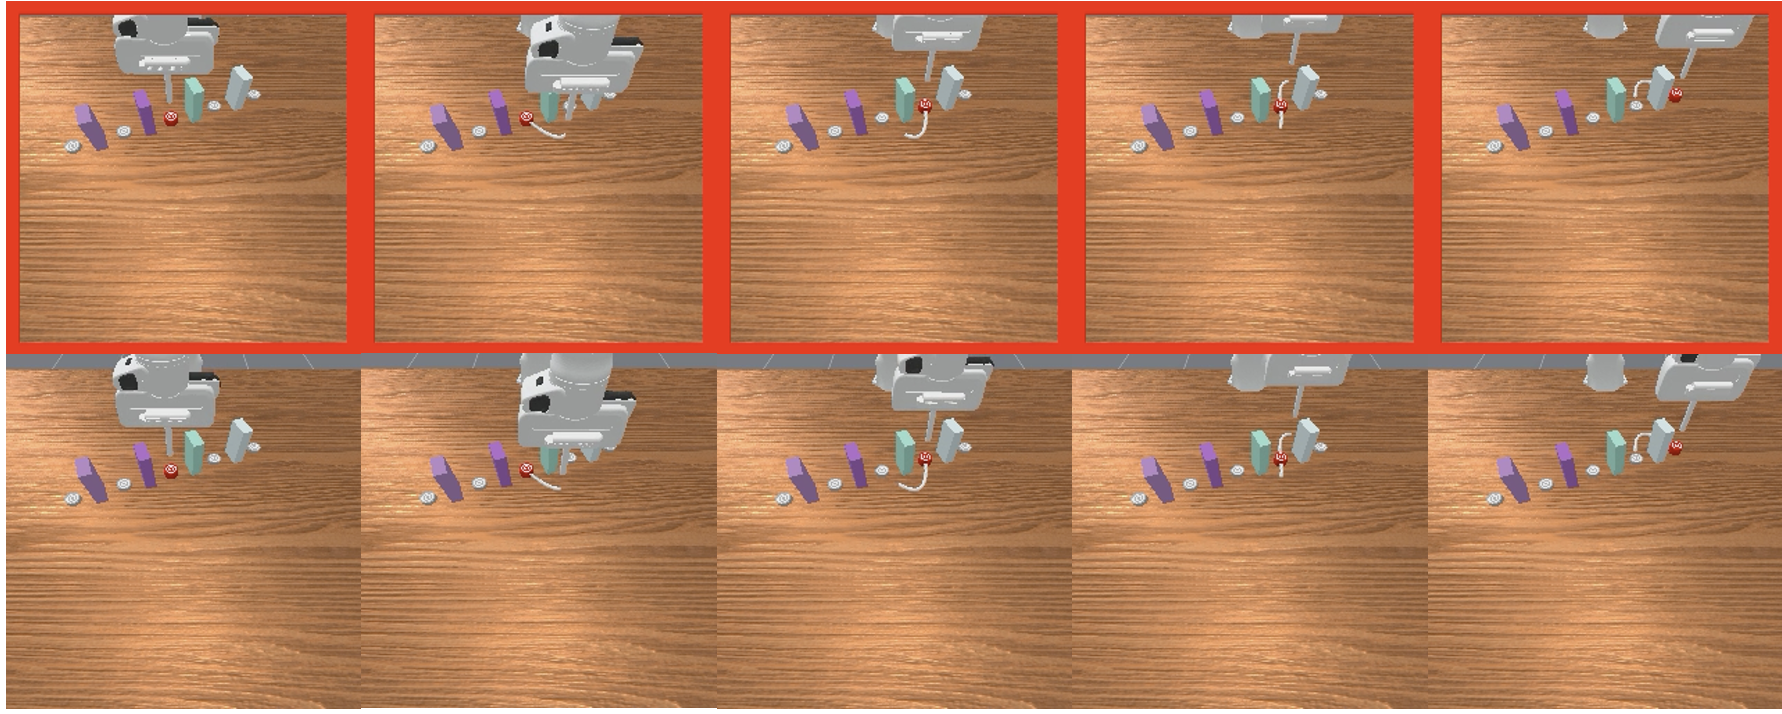
\includegraphics[width=1\linewidth]{images/tasks/routestick.png}
    \caption{\textbf{RouteStick Task Example.} In this instance, the robot watches the video and uses the stick attached to the end-effector to navigate around obstacles on the table, reproducing the demonstrated path.}
    \label{fig:routestick}
\end{figure}


\paragraph{Language Goal} \textit{``Watch the video carefully, then use the stick attached to the robot to navigate around the obstacles on the table, following the same path shown in the video.''}

\paragraph{Task Characteristics}

Each episode consists of a \textbf{video phase} and an \textbf{execution phase}.

\begin{itemize}[itemsep=1pt, topsep=0pt, leftmargin=*]

    \item \textbf{Video:} The robot navigates with a stick around fixed obstacles and visits targets in sequence, implicitly specifying clockwise or counterclockwise circling directions.

    \item \textbf{Execution:} After reset, the robot must visit the same targets in the same order and match the demonstrated circling directions continually. The environment provides real-time visual feedback during execution:
    \begin{itemize}[itemsep=1pt, topsep=0pt, leftmargin=*]
        \item \textbf{Target highlighting feedback:} A target turns red when visited by the stick, indicating successful contact.
        \item \textbf{Trajectory trace feedback:} A line continuously renders the stick-tip trajectory in real time.
    \end{itemize}

\end{itemize}


\paragraph{Success Criteria}

\begin{itemize}[itemsep=1pt, topsep=0pt, leftmargin=*]

    \item \textbf{Correct completion:} The robot visits all targets in the demonstrated order, matches each obstacle-circling direction (clockwise/counterclockwise), and maintains a continuous trajectory.

    \item \textbf{Immediate failure:} the episode terminates early if the robot deviates from the demonstrated order.
\end{itemize}
